\documentclass[12pt,letterpaper,noanswers]{exam}
%\usepackage{color}
\usepackage[usenames,dvipsnames,svgnames,table]{xcolor}
\usepackage[margin=0.9in]{geometry}
\renewcommand{\familydefault}{\sfdefault}
\usepackage{multicol}
%\newcommand{\mathbf}[1]{\boldsymbol{#1}}
\pagestyle{head}
\definecolor{c02}{HTML}{FFBBBB}
\definecolor{c03}{HTML}{FFDDDD}
\header{AM 111 Problem Set 05}{}{{\colorbox{c02}{\makebox[2.8cm][l]{Due Fri Oct 20}}}\\at 12pm}
\runningheadrule
\headrule
\usepackage{diagbox}
\usepackage{graphicx} % more modern

\usepackage{amsmath} 
\usepackage{amssymb} 

\usepackage{hyperref}

\usepackage{tcolorbox}
\usepackage[framed,numbered,autolinebreaks,useliterate]{mcode}


\def\been{\begin{enumerate}}
\def\enen{\end{enumerate}}
\def\beit{\begin{itemize}}
\def\enit{\end{itemize}}
\def\dsst{\displaystyle}
\def\dx{\Delta x}
\hyphenation{}
\newcommand{\blank}[1]{\underline{\hspace{#1}}}

\makeatletter
\newcommand{\pyf}{%
  \begingroup\catcode`_=12
  \pyf@
}
\newcommand{\pyf@}[1]{\texttt{#1}\endgroup}
\makeatother

\newcommand{\note}[1]{\textcolor{red}{#1}} % show notes in red
%\renewcommand{\note}[1]{} % don't display notes


\begin{document}
 \pdfpageheight 11in 
  \pdfpagewidth 8.5in

\begin{itemize}
    \itemsep0pt
    \item Find the \href{https://github.com/sarah1123/ScientificComputing-APMTH111/blob/main/2023Fall/PythonFiles/05_interpolation/ProblemSet05.ipynb}{ProblemSet05 Python template} via this link.
    \item Use this python notebook for all programming work on the problem set.  Submit the notebook to the Python assignment on Gradescope.
    \item Submit the other problems to the pdf assignment on Gradescope.
    \item Late work: Problem sets are due at noon on Fridays.  They are accepted until 5pm for all students without penalty.  In addition, you have three 29-hour late days that allow you to submit until 5pm on Saturday.  You don't need to ask to use your late days, just keep track of them for yourself.
\end{itemize}


% NOTES:
% splits this problem set into implementation and Runge phenomenon, exploration?, and application.

\begin{questions}
\question (Projects) This problem is a first exploration of papers related to numerical analysis and scientific computing topics.

Your project work will be based on a paper in one of these areas.  You can do further exploration beyond this assignment as you look for topics for your project.

This assignment involves making three discussion board posts.


\begin{parts}
\item Choose one of the papers from the paper list accompanying this problem set.  The papers are all drawn from the SIAM Review Education section.  They are typically not research papers, but are instead are written for exposition/education on an applied math topic.


\emph{SIAM is the Society for Industrial and Applied Mathematics}.

Most of them veer towards the numerical analysis side, rather than focusing on scientific problems being solved by computing.
    
Once you have opened the paper, work to read the abstracts, read part of the introduction, and look through the equations, diagrams, and figures in the paper.  Identify the main problem being tackled in the paper.


Post to the PSet 05 Q1a Discussion Board on Canvas.  If another student has already posted about the paper, then make your post within the same thread as theirs.  In your post, give the title of the paper, and make a comment about the abstract.  Mention something you found interesting, something you didn't understand, and something else that you would like to share.


\item Do a search for a published paper that connects to a topic you are interested in and involves numerical simulation or the use of computational methods.  The paper can be methods-focused or focused on an application while making use of numerical methods or simulations.

Read the abstract, read part of the introduction, and look through the equations, diagrams, and figures in the paper.  Identify the main question being explored or answered in the paper.

To do the search you might use \url{https://scholar.google.com} or another scientific index.  If you use an index besides Google Scholar, mention it in your post.    
    

Post to the PSet 05 Q1b Discussion Board on Canvas.  In your post, give the title, authors, and year of the paper.  Share how you found the paper, what led you to choose it, an unfamiliar term that you saw in the abstract or paper, and anything else that you would like to share.

\item Browse the posts for Q1a and Q1b written by other students.  Based on their posts, choose one additional paper to read.  Again read the abstract, read part of the introduction, and look through the equations, diagrams, and figures in the paper.  Then reply to the post with (i) what drew you to choose this paper and (ii) additional information about the paper (something you found interesting that hasn't already been mentioned, etc).

\end{parts}  


\item (Lagrange interpolation implementation) 

Find the HumpherysJarvisBYU-ACME-LabsVolume2.pdf in the Additional Materials folder in the Files on Canvas.

In the Polynomial Interpolation section, 
\begin{parts}
\item Read Problem 1.  Write \pyf{lagrangehelper(xdata, ydata, xinterp)}, to call from within \texttt{lagrange}.  

Notice the note to use the functions \texttt{np.prod()} and \texttt{np.delete()} as part of your method.
\item Complete Problem 2.
\item Test your function by using it to make the plots from 9.1 (as suggested in Problem 2).
\end{parts}

\item (cubic spline interpolation implementation) (From Koumoutsakos et al Notebook 5)

You'll write a code to perform cubic spline interpolation for four data points (also called nodes or knots). The points are $(0,1), (1,0), (2,0.3), (3,0)$.


See Sauer \S 3.4 for formula references.
\begin{itemize}
    \item $\delta_i = x_{i+1}-x_i$
    \item $\Delta_i = y_{i+1}-y_i$
    \item $S_i(x) = y_i + b_i(x-x_i) + c_i(x-x_i)^2 + d_i(x-x_i)^3$ on $[x_i,x_{i+1}]$
    \item $d_i = \frac{c_{i+1}-c_i}{3\delta_i}$
    \item $b_i = \frac{\Delta_i}{\delta_i} - \frac{\delta_i}{3}(2c_i + c_{i+1})$
\end{itemize}


\begin{parts}
\item Using the natural cubic splines assumption (i.e. $c_1 = S_1''(x_1) = 0$ and $c_4 = S_3''(x_) = 0)$, construct the system of equations to find the $c_i$ values.  

See the class handout for the equation to use for $c_i$.







\item Create a function called \texttt{cubic(x,xi,xi1,yi,yi1,ci,ci1)} that returns the values of the cubic polynomial, $S_i(x)$, at the array of input points \texttt{x}.

\begin{itemize}
\item \texttt{x} is an array of evaluation points for the cubic
\item \texttt{xi} is $x_i$
\item \texttt{xi1} is $x_{i+1}$
\item \texttt{yi} is $y_i$
\item \texttt{yi1} is $y_{i+1}$
\item \texttt{ci} is $c_i$
\item \texttt{ci1} is $c_{i+1}$
\end{itemize}


\item Solve the system from part (a) using a \texttt{numpy} function such as \texttt{np.linalg.solve}.  

Generate $20$ interpolation points between the endpoints of each $S_i$.  Use \texttt{cubic} to evaluate $S_i$ at these points.  Create a plot of the graph of your interpolating function.

\item Assess your interpolating function.  Is it continuous?  Based on your plot, does it appear to have continuous first and second derivatives?

\item Revise your matrix equation from part (a) for the case where the left end is clamped (leave the right side natural).  

Set $S_1'(x_1) = 0$.  Use this condition to find an equation in terms of the $c_i$.

\item Solve and plot the results.  Use the interpolation points you generated above.

\item Now adjust the system so that both ends are clamped.  

\item Solve and plot as above.

\item Make a system of equations for the parabolic rollout conditions ($S_1''(x_1) = S_1''(x_2)$ and $S_{n-1}''(x_{n-1}) = f_{n-1}''(x_n)$.  

\item Solve and plot as above.


\end{parts}

\item (Sauer \S3.4 Computer 14) Compile a list of 101 consecutive daily close prices of an exchange-traded stock from a financial data website.

\emph{I expect no two students to use the same data for this, given the large space of possible datasets.}

\begin{parts}
\item Create an interpolating polynomial that passes through every fifth point of the time series (day $0,5,10,...,100$).  Plot the degree 20 interpolating polynomial along with the daily data.  

\item Construct, and plot, the natural cubic spline with interpolating nodes $0:5:100$, along with the daily data.

\emph{Use} \texttt{scipy.interpolate.CubicSpline} \emph{to create your spline fit.}
\item What is the maximum interpolation error for each method?

Is the Runge phenomenon of oscillation need the edges visible in your plot?

Compare the two approaches of representing the data.
\end{parts}

\item \emph{Time permitting} 
(Chebyshev points)

In the HumpherysJarvisBYU-ACME-LabsVolume2.pdf in the Additional Materials folder in the Files on Canvas, within the Polynomial Interpolation section, complete Lab 9 problem 5

\item \emph{Time permitting} (Greenbaum and Chartier \S 8.8 15)

Follow the steps below to fit a two-dimensional cubic spline (a bi-cubic spline) through this altitude data and plot the result.

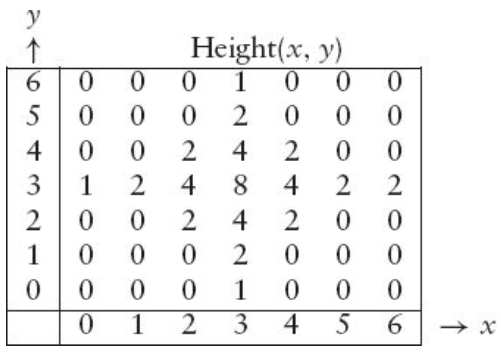
\includegraphics[width=3in]{img/PSet05hill.png}

\begin{parts}
\item Fit a not-a-knot cubic spline to the data in each row.  Then evaluate at the points $x = 0,0.1,0.2,...,5.9,6.0$ to create a $7\times 61$ array of values.

\emph{Use} \texttt{scipy.interpolate.CubicSpline} \emph{to create your spline fit.}
\item Fit a not-a-knot cubic spline to the data in each column of your $7\times 61$ array.  Evaluate these at $y = 0.0,0.1,0.2,...,5.9,6.0$ to produce a $61\times 61$ array of values.  Call this matrix $M$.
\item The code below has examples of two different ways to plot data from a 2D array.  Try each method for your data.
\begin{verbatim}
import numpy as np
from matplotlib import pyplot as plt
data = np.random.rand(61, 61)

# plot as an image
plt.imshow(data)
plt.show()

# surface plot
ax = plt.axes(projection='3d')
xvals = np.linspace(0,1,61)
x,y = np.meshgrid(xvals,xvals)
ax.plot_surface(x, y, data)
\end{verbatim}
\end{parts}


\item \emph{Time permitting} (Greenbaum and Chartier \S8.8 16)

PostScript and TrueType letters are created with splines using only a few points for each letter.  


The following code creates a letter from 7 data points.
\begin{verbatim}
import numpy as np
from scipy.interpolate import CubicSpline
import matplotlib.pyplot as plt

x = np.array([1, 2, 3, 2, 1.2, 2, 2.7])
y = np.array([1, 0, 1, 2.5, 3.4, 4, 3.2])
n = len(x)
t = np.arange(n)
delta = 0.01
tt = np.arange(0,n-1+delta,delta)
fx = CubicSpline(t,x)
fy = CubicSpline(t,y)

fig, ax = plt.subplots(1,1)
plt.plot(x,y,'o')
plt.plot(fx(tt),fy(tt))
ax.set_aspect('equal', 'box')    
\end{verbatim}

\begin{parts}
\item Create and print the letter defined by the following data.

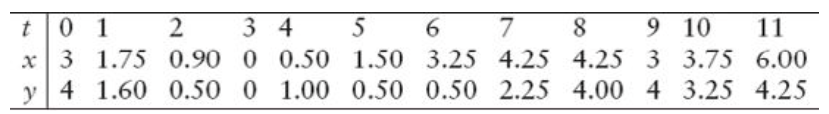
\includegraphics[width=0.6\textwidth]{img/PSet05letterdata.png}

\item On the same axes plot this letter along with the letter doubled in size.

\emph{\texttt{2*x} will double the size of the font in the $x$-direction.}

\item Create and print a different script letter.

\emph{Generate the $(t,x,y)$ values yourself - it's fine if your letter looks a little rough.}
\end{parts}









\question Reflection
\begin{parts}
\item When you worked on the problem set where did you get stuck or become confused?
\item What aspects of the course challenged you this week?  What did you do to address those challenges?  What topics/ideas/procedures do you not yet understand?
\item What did you understand the best this week?  What, if anything, do you understand better this week than you did in the past?
\item List the people that you worked with or consulted on the problem set problems.  This might include other students in the course, course instructors, or people who have previously taken the course.
\item Below, indicate how much of your time for this class has been doing the following activities:
	\begin{enumerate}
	\item Working on the problem set (including time in Python)
	\item Reviewing course materials, including the course textbooks
	\item Working through supplementary materials
	\item Going to office hours or lab
	\item Other (please specify)
	\end{enumerate}
\item If you used chatGPT or other AI tools, attach that information as part of this question.
\end{parts}

\end{questions}

\noindent\textbf{Extra information}

The structure of the final project:

 It will be based on a published paper.  You will work to understand and replicate key results.  Depending on the breadth and depth of the paper you will be expected to create a small extension or do a different exploration.
 
 I am providing a list of possible papers for this (\emph{see attached list}), or you can propose a paper.  There will be only one team per paper.

The default for the project will be to work in a team of three.  If there's a reason that a group of one, two, or four would work better, you'll have a chance to speak with me about arranging an exception. 

The teams will be assigned and the project proposals will be due later in October. %\textbf{Monday, April 1st}.  

A timeline for the project deliverables and more detailed expectations will be included in the next problem set.


\end{document}